% ============================================================
%  Balancing Robot – Systemdokumentation
%  Design: AR10-inspiriert (Blau, Sidebar, Kapiteltrennseiten)
%  Compiler: pdflatex (2× laufen lassen)
% ============================================================

\documentclass[11pt, a4paper, twoside=false]{scrbook}

% ── Pakete ──────────────────────────────────────────────────
\usepackage[T1]{fontenc}
\usepackage[utf8]{inputenc}
\usepackage[ngerman]{babel}
\usepackage{lmodern}
\usepackage{microtype}

\usepackage[a4paper,
  top=25mm, bottom=30mm,
  left=22mm, right=22mm,
  includeheadfoot]{geometry}

\usepackage{xcolor}
\usepackage{graphicx}
\usepackage{tikz}
\usetikzlibrary{calc}
\usepackage{tcolorbox}
\tcbuselibrary{skins, breakable}
\usepackage{titlesec}
\usepackage{fancyhdr}
\usepackage{setspace}
\usepackage{enumitem}
\usepackage{booktabs}
\usepackage{hyperref}
\usepackage{listings}
\usepackage{amsmath}

% ── Farben ──────────────────────────────────────────────────
\definecolor{htbblue}{HTML}{0078C8}      % Hauptblau (AR10-ähnlich)
\definecolor{htbdark}{HTML}{003E6B}      % Dunkelblau für Akzente
\definecolor{htblight}{HTML}{E8F4FC}     % Hellblau für Hintergründe
\definecolor{htbgray}{HTML}{F4F4F4}      % Hellgrau
\definecolor{htbtextgray}{HTML}{555555}  % Grauer Fließtext

% ── Schrift ─────────────────────────────────────────────────
\usepackage{helvet}
\renewcommand{\familydefault}{\sfdefault}   % Sans-serif durchgehend

% ── Hyperlinks ──────────────────────────────────────────────
\hypersetup{
  colorlinks=true,
  linkcolor=htbblue,
  urlcolor=htbblue,
  citecolor=htbblue,
  pdfauthor={HTW Berlin – Industrielle Robotik WiSe 25},
  pdftitle={Balancing Robot – Systemdokumentation},
}

% ── Listings (Code) ─────────────────────────────────────────
\lstset{
  basicstyle=\ttfamily\small,
  keywordstyle=\color{htbblue}\bfseries,
  commentstyle=\color{htbtextgray}\itshape,
  stringstyle=\color{htbdark},
  backgroundcolor=\color{htbgray},
  frame=single, framerule=0pt,
  rulecolor=\color{htblight},
  numbers=left, numberstyle=\tiny\color{htbtextgray},
  breaklines=true,
  showstringspaces=false,
  tabsize=4,
}

% ── Kopf- und Fußzeile ──────────────────────────────────────
\pagestyle{fancy}
\fancyhf{}
\renewcommand{\headrulewidth}{0pt}
\fancyhead[L]{%
  \begin{tikzpicture}[remember picture, overlay]
    \fill[htbblue] (0,0) rectangle (\textwidth+4mm, 7mm);
    \node[anchor=west, white, font=\small\bfseries] at (2mm,3.5mm)
      {Balancing Robot – Systemdokumentation};
    \node[anchor=east, white, font=\small] at (\textwidth+2mm,3.5mm)
      {\thepage};
  \end{tikzpicture}%
}
\setlength{\headheight}{10mm}

% Erste Seite eines Kapitels: nur Seitenzahl unten
\fancypagestyle{plain}{%
  \fancyhf{}
  \renewcommand{\headrulewidth}{0pt}
  \fancyfoot[C]{\color{htbtextgray}\small\thepage}
}

% ── Kapitelüberschriften ─────────────────────────────────────
%   Blaue Box links + große Kapitelnummer
\titleformat{\chapter}[block]
  {\normalfont\Huge\bfseries}
  {}
  {0pt}
  {%
    \begin{tcolorbox}[
      enhanced, sharp corners,
      colback=htbblue, colframe=htbblue,
      left=6mm, right=6mm, top=4mm, bottom=4mm,
      width=\textwidth,
    ]
      \color{white}%
      \raisebox{0pt}[\height][0pt]{%
        \makebox[0pt][r]{%
          \fontsize{60}{60}\selectfont\color{white!30!htbblue}%
          \thechapter\hspace{4mm}%
        }%
      }%
      #1
    \end{tcolorbox}%
  }
\titlespacing*{\chapter}{0pt}{-20pt}{20pt}

% Abschnittsüberschriften
\titleformat{\section}
  {\color{htbblue}\large\bfseries}
  {\thesection}
  {1em}{}
  [\color{htbblue}\titlerule[0.6pt]]

\titleformat{\subsection}
  {\color{htbdark}\normalsize\bfseries}
  {\thesubsection}
  {1em}{}

% ── Info-Box (tcolorbox) ────────────────────────────────────
\newtcolorbox{infobox}[1][]{
  enhanced, breakable,
  colback=htblight, colframe=htbblue,
  leftrule=4pt, toprule=0pt, bottomrule=0pt, rightrule=0pt,
  sharp corners,
  title=#1, fonttitle=\bfseries\color{htbblue},
  #1
}

% ── Kapiteltrennseite ────────────────────────────────────────
%   Aufruf: \chapterpage{Kapitel-Nr}{Titel}{Kurzbeschreibung}
\newcommand{\chapterpage}[3]{%
  \clearpage
  \thispagestyle{empty}
  \begin{tikzpicture}[remember picture, overlay]
    % Vollfläche Blau
    \fill[htbblue] (current page.south west) rectangle (current page.north east);
    % Große blasse Kapitelnummer im Hintergrund
    \node[anchor=east, opacity=0.15, white,
          font=\fontsize{200}{200}\selectfont\bfseries]
      at ([xshift=-10mm]current page.east |- current page.center) {#1};
    % Horizontale Linie
    \draw[white, line width=1pt]
      ([xshift=20mm, yshift=15mm]current page.west |- current page.center)
      -- ([xshift=-20mm, yshift=15mm]current page.east |- current page.center);
    % Kapiteltext
    \node[anchor=west, white, font=\Huge\bfseries, text width=160mm]
      at ([xshift=20mm, yshift=25mm]current page.west |- current page.center) {#2};
    % Beschreibungstext
    \node[anchor=west, white, opacity=0.85, font=\large, text width=150mm]
      at ([xshift=20mm, yshift=2mm]current page.west |- current page.center) {#3};
    % Vertikaler Sidebar-Text links
    \node[anchor=south, rotate=90, white, opacity=0.5, font=\small\bfseries]
      at ([xshift=10mm]current page.west |- current page.center)
      {BALANCING ROBOT · HTW Berlin · WiSe 25};
  \end{tikzpicture}
  \clearpage
}

% ============================================================
\begin{document}

% ── Titelseite (AR10-Stil) ───────────────────────────────────
%
%  Obere ~55 %: blauer Block
%    – Roboterbild (Linienstil) oben links, leicht überlappend
%    – Titel groß, unten rechts im blauen Block
%    – Untertitel kleiner, darunter
%
%  Untere ~45 %: weißer Block
%    – Dokumenttyp fett oben links
%    – Projektname darunter
%    – HTW-Logo unten rechts
%
%  Bilder ersetzen:
%    robot_cover.png  → Foto/Render eures Roboters (beliebige Größe,
%                        wird auf 90 mm Breite skaliert)
%    htw_logo.png     → HTW-Berlin-Logo (transparenter Hintergrund)
%
\begin{titlepage}
  \newgeometry{margin=0pt}   % keine Seitenränder auf der Titelseite
  \begin{tikzpicture}[remember picture, overlay]

    % ── Blauer oberer Block (55 % der Seite) ──────────────────
    \fill[htbblue]
      (current page.north west)
      rectangle
      ([yshift=-0.55\paperheight]current page.north east);

    % ── Roboterbild oben links ─────────────────────────────────
    %   Platzhalter-Rahmen: durch \includegraphics ersetzen
    \node[anchor=north west]
      at ([xshift=10mm, yshift=-8mm]current page.north west)
      {%
        % robot_cover.png (transparenter Hintergrund) hat Vorrang vor .jpg
        \IfFileExists{robot_cover.png}{%
          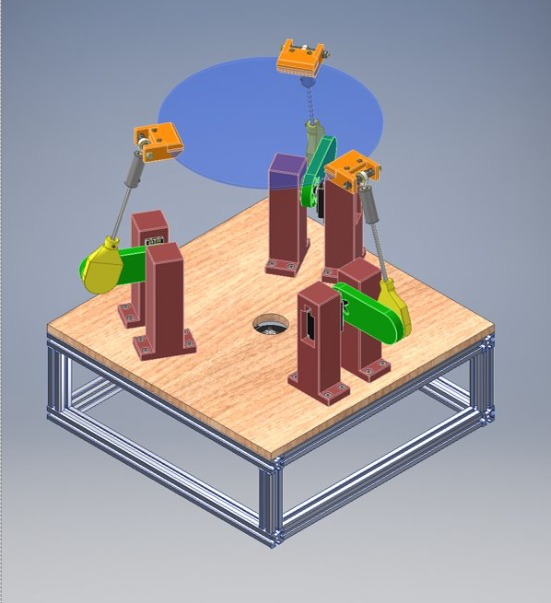
\includegraphics[width=90mm, keepaspectratio]{robot_cover.png}%
        }{%
          \IfFileExists{robot_cover.jpg}{%
            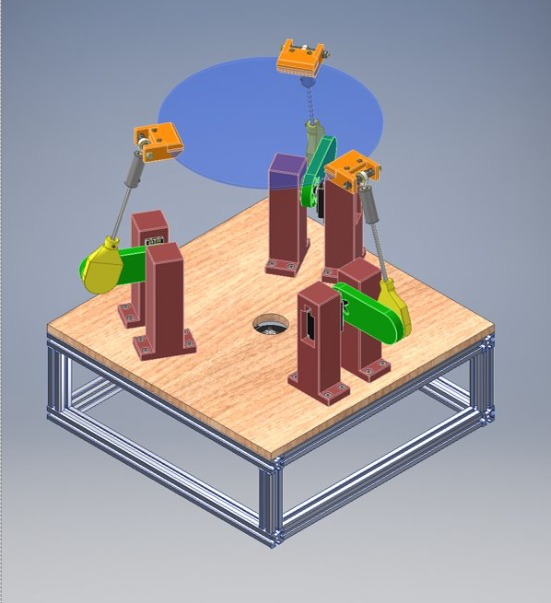
\includegraphics[width=90mm, keepaspectratio]{robot_cover.jpg}%
          }{%
            \begin{tikzpicture}
              \draw[white, dashed, line width=1pt, opacity=0.4]
                (0,0) rectangle (90mm, 110mm);
              \node[white, opacity=0.5, font=\small] at (45mm,55mm)
                {robot\_cover.png/.jpg};
            \end{tikzpicture}%
          }%
        }%
      };

    % ── Titel unten rechts im blauen Block ────────────────────
    \node[anchor=south east, align=right]
      at ([xshift=-14mm, yshift=12mm]current page.north east |-
          [yshift=-0.55\paperheight]current page.north)
      {%
        {\fontsize{36}{40}\selectfont\bfseries\color{white}Balancing Robot}\\[4pt]
        {\large\bfseries\color{white!85!htbblue}Systemdokumentation}%
      };

    % ── Weißer unterer Block ──────────────────────────────────
    % (Hintergrund ist bereits weiß; nur Texte positionieren)

    % Dokumenttyp + Projektname
    \node[anchor=north west, align=left]
      at ([xshift=14mm, yshift=-10mm]current page.south west |-
          [yshift=-0.55\paperheight]current page.north)
      {%
        {\large\bfseries\color{black}Systemdokumentation}\\[4pt]
        {\normalsize\color{htbtextgray}Balancing Robot · HTW Berlin · WiSe 2025/26}%
      };

    % HTW-Logo unten rechts
    \node[anchor=south east]
      at ([xshift=-14mm, yshift=14mm]current page.south east)
      {%
        \IfFileExists{htw_logo.png}{%
          
\includegraphics[height=18mm, keepaspectratio]{htw_logo.png}%
        }{%
          \begin{tikzpicture}
            \draw[htbblue, dashed, line width=0.8pt, opacity=0.5]
              (0,0) rectangle (40mm,16mm);
            \node[htbblue, opacity=0.6, font=\small] at (20mm,8mm)
              {htw\_logo.png};
          \end{tikzpicture}%
        }%
      };

  \end{tikzpicture}
  \restoregeometry
\end{titlepage}

% ── Vorwort / Inhaltsverzeichnis ────────────────────────────
\frontmatter
\tableofcontents
\clearpage

% ============================================================
\mainmatter

% ── Kapitel 1 ────────────────────────────────────────────────
\chapterpage{1}{Systemübersicht}{Aufbau, Ziel und Komponenten des Balancing Robots}

\chapter{Systemübersicht}

\section{Projektziel}

Der Balancing Robot ist eine dreiachsig steuerbare Plattform, die einen Ball
durch gezielte Neigung in einer Zielposition balanciert. Das System kombiniert
Mechanik, Servoansteuerung, Inverse Kinematik und Computer Vision.

\begin{infobox}[Kernfunktion]
  Kamera erkennt Ballposition → PD-Regler berechnet Sollwinkel →
  Inverse Kinematik bestimmt Servowinkel → Plattform neigt sich.
\end{infobox}

\section{Systemarchitektur}

% Platzhalter für Blockdiagramm
\begin{figure}[h]
  \centering
  \fbox{\parbox{0.8\textwidth}{\centering\vspace{20mm}
    [Blockdiagramm: Vision → Regler → Kinematik → Hardware]
  \vspace{20mm}}}
  \caption{Systemarchitektur des Balancing Robots}
\end{figure}

\section{Hardwarekomponenten}

\begin{table}[h]
  \centering
  \begin{tabular}{lll}
    \toprule
    \textbf{Komponente} & \textbf{Typ} & \textbf{Beschreibung} \\
    \midrule
    Raspberry Pi     & 4B (4 GB)       & Hauptrechner \\
    Servos           & MG996R (×3)     & Plattformantrieb \\
    Servo-Controller & PCA9685         & I²C PWM-Board \\
    Kamera           & Pi Camera v2    & Ballerfassung \\
    Plattform        & 3-Bein-Delta    & Parallele Kinematik \\
    \bottomrule
  \end{tabular}
  \caption{Hardwarekomponenten}
\end{table}

% ── Kapitel 2 ────────────────────────────────────────────────
\chapterpage{2}{Mechanik \& Kinematik}{Geometrie der Plattform und Inverse Kinematik}

\chapter{Mechanik und Kinematik}

\section{Plattformgeometrie}

% ... hier Inhalt einfügen ...

\section{Inverse Kinematik}

% ... hier Inhalt einfügen ...

% ── Kapitel 3 ────────────────────────────────────────────────
\chapterpage{3}{Computer Vision}{Kamerakalibrierung und Ballerkennung}

\chapter{Computer Vision}

\section{Kamerakalibrierung}

% ... hier Inhalt einfügen ...

\section{Ballerkennung}

% ... hier Inhalt einfügen ...

% ── Kapitel 4 ────────────────────────────────────────────────
\chapterpage{4}{Regelung}{PD-Regler und Systemintegration}

\chapter{Regelung}

\section{PD-Regler}

% ... hier Inhalt einfügen ...

% ============================================================
\backmatter

\end{document}
